\documentclass{article}
\usepackage{booktabs}
\usepackage{amsmath}
\usepackage{algorithmic}
\usepackage[nothing]{algorithm}
\usepackage{tikz}
\providecommand{\e}[1]{\ensuremath{\times 10^{#1}}}
\renewcommand{\thealgorithm}{}
\title{CS 521: Data Structures and Algorithms I \\ Homework 3}
\author{Dustin Ingram}
\begin{document}
\maketitle
\begin{enumerate}
\item \textbf{Solution:}
\begin{itemize}
    \item \textbf{Adjacency-list:} For every vertex in a given vertex's adjacency-list, this algorithm traverses it's respective adjacency list (two edges away) to compute the square:
    \begin{algorithm}[H]
    \floatname{algorithm}{Adjacency-Square}
    \caption{}
    \begin{algorithmic}
    \FOR{$V \in G$} 
    \FOR{$V' \in G.Adj[V]$} 
    \FOR{$V'' \in G.Adj[V']$} 
    \IF{$V \neq V''$}
    \STATE $G[V].append(V'')$ 
    \ENDIF
    \ENDFOR
    \ENDFOR
    \ENDFOR
    \end{algorithmic} 
    \end{algorithm}
Because this algorithm operates on the adjacencies-of-adjacencies, the running time is given by $O(V^{3})$.
    \item \textbf{Adjacency-matrix:} Similar to the previous algorithm, this algorithm travels two hops away from a given vertex. Since an adjacency-matrix gives us a $1$ if there is an edge and a $0$ if there is not, we can use this to our advantage -- if both are $1$, we add $1$ to $G(i,j)$, otherwise we add $0$.
    \begin{algorithm}[H]
    \floatname{algorithm}{Matrix-Square}
    \caption{}
    \begin{algorithmic}
    \FOR{$i = 1 \dots V$}
    \FOR{$j = 1 \dots V$}
    \FOR{$j' = 1 \dots V$}
    \IF{$i \neq j$}
    \STATE $G(i,j) = G(i,j) + (G(i,j') \times G(j,j'))$
    \ENDIF
    \ENDFOR
    \ENDFOR
    \ENDFOR
    \end{algorithmic} 
    \end{algorithm}
    The three nested loops result in a running time of $O(V^{3})$.
\end{itemize}
\item \textbf{Solution:} 
The entries of the matrix product $BB^{T}$ (where $B^{T}$ is the transpose of $B$ and $B$ is the incidence matrix of a directed graph $G = (V,E)$) are represented such that
\begin{equation*}
|BB^{T}(i,j)|= 
\begin{cases} \text{Degree of $i$} & \text{if $i=j$,}
\\
\text{Number of edges between $i$ and $j$} & \text{if $i\neq j$.}
\end{cases}
\end{equation*}

\item \textbf{Solution:} 
\begin{itemize}
    \item \textbf{Adjacency-list:}
    The adjacency-list algorithm passes through each vertex $V$ in $G(V,E)$, adding $V$ to the adjacency list of $G^{T}$ for each adjacent vertex:
    \begin{algorithm}[H]
    \floatname{algorithm}{Adjacency-Transpose}
    \caption{}
    \begin{algorithmic}
    \FOR{$V \in G$} 
    \FOR{$V' \in G.Adj[V]$} 
    \STATE $G^{T}[V'] = V$ 
    \ENDFOR
    \ENDFOR
    \end{algorithmic} 
    \end{algorithm}
    This iterates through V vertices and each of their roughly $\frac{E}{V}$ adjacent vertices, for a total runtime of $O(V+E)$.

    \item \textbf{Adjacency-matrix:}
    Since $G$ is represented by a square $V\times{V}$ matrix, this is simply the transposition of the matrix. Since this algorithm visits every element in the matrix, it runs in $O(V^{2})$ time. 
    \begin{algorithm}[H]
    \floatname{algorithm}{Matrix-Transpose}
    \caption{}
    \begin{algorithmic}
    \FOR{$i = 1 \dots V-1$} 
    \FOR{$j = i+1 \dots V$} 
    \STATE $G^{T}(i,j) = G(j,i)$ 
    \ENDFOR
    \ENDFOR
    \end{algorithmic} 
    \end{algorithm}
If we do not need to produce a new matrix $G^{T}$, however, we can use $G$ as $G^{T}$ simply by inverting the indices, i.e. since $G(i,j)=G^{T}(j,i)$, we can produce any value in $G^{T}$ in $O(1)$.

\end{itemize}

\item \textbf{Solution:}
Here, $(u,v)$ is a safe edge for $A$, as it will eventually become part of the MST of $G$, however, in this iteration (after $(a,u)$ has been added to the MST) it is not a light edge (a minimum edge crossing $S$ and $V-S$). 
\begin{figure}[!h]
\centering
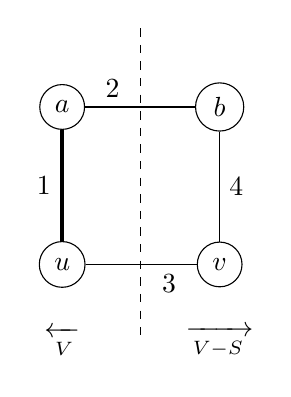
\begin{tikzpicture}[]
  \node[draw,shape=circle]     (a) at (0,0)  {$a$};
  \node[draw,shape=circle]     (b) at (2,0)  {$b$};
  \node[draw,shape=circle]     (u) at (0,-2) {$u$};
  \node[draw,shape=circle]     (v) at (2,-2) {$v$};
  \node (s) at (0,-3) {$\xleftarrow[V]{}$};
  \node (vs) at (2,-3) {$\xrightarrow[V-S]{}$};

  \draw (a) -- (b) node[near start,above] {2};
  \draw[ultra thick] (a) -- (u) node[midway, left] {1};
  \draw (b) -- (v) node[midway, right] {4};
  \draw (u) -- (v) node[near end, below] {3};
  \draw[dashed] (1,1) -- (1,-3);
\end{tikzpicture}
\end{figure}

\item \textbf{Solution:} 
Decreasing the weight of an edge in $T$, the MST of $G$, still satisfies the two properties of an MST:
\begin{enumerate}
    \item All vertices in $G$ are connected in $T'$;
    \item The sum of the edges of $T'$ are the minimum possible combination of edges to maintain (a).
\end{enumerate}
More formally, this definition maintains the edge weights of $T$ if the edge is not $(x,y)$ and if it is $(x,y)$, subtracts $k$ from this single edge. As long as $k > w(x,y)$, (thus making $w'(u,v)$ negative), this holds.

\item \textbf{Solution:} 
If the graph $G(E,V)$ already has a minimum spanning tree $T$ computed, the speed at which we can update the MST if we add a new vertex $v'$ and it's incident edges $E'$ to $G$ depends on two variables: the number of vertices in $T$, and the number of incident edges to be added.\\
For a base case, consider that $E'=1$, i.e., that a single vertex $v'$ and a single edge to \emph{some} vertex in $T$ is added. Since this single edge is the only possible path to $v'$, it must become a part of the MST.\\
If there are more than one incident edges in $E'$, any of these edges will induce a cycle in $T$ (after the first minimum edge is added), with the maximally weighted edge in the cycle not necessarily being an incident edge. Additionally, there can be at most $V$ incident edges (if there were one to every vertex $V$ in $T$). \\
If we add every incident edge in $E'$ to the edges in $T$ (which can be at most $V-1$ edges), this results in a graph with at most $2V-1$ edges. We can run either Kruskal's or Prim's algorithm on the resulting graph to produce the MST, which will run in $O(E\lg{V})$, but since we know $E$ of this new graph can be no more than $2V-1$, this is in fact $O(V\lg{V})$.

\item \textbf{Solution:}
We can use the figure from solution 4 for this problem as well. If we partition the graph $G$ into subgraphs such that ${a, u} \in V_{1}$ and ${b, v} \in V_{2}$, recursively solving the MST for these subgraphs will result in adding the edge $(a,u)$ to $V_{1}$ and similarly $(b,v)$ to $V_{2}$. It is clear that adding $(a,b)$, the light edge crossing the cut will not produce an MST.

\end{enumerate}
\end{document}
